\documentclass[10pt,a4paper]{article}
\usepackage[english]{babel}
\usepackage[utf8]{inputenc}
\usepackage{amsmath}
\usepackage{amsfonts}
\usepackage{amssymb}
\usepackage{graphicx}
\usepackage{float}
\usepackage{caption}

%link to documentation: 
%https://ackrep-doc.readthedocs.io/en/latest/devdoc/contributing_data.html

\begin{document}
	\part*{Model Documentation of the \\ Overhead Crane} % MUST - Add Model Name 
	
	%%%%%%%%%%%%%%%%%%%%%% NOMENCLATURE %%%%%%%%%%%%%%%%%%%%%%%%%%%
	
	\section{Nomenclature} % MUST
	\subsection{Nomenclature for Model Equations} % MUST
	
	%variables for model equations
	\begin{tabular}{ll}
		$s_1$ & center of gravity distance of the load \\
		$m_1$ & mass of trolley 1 \\
		$m_2$ & mass of load \\
		$m_3$ & mass of trolley 2 \\
		$J_2$ & moment of inertia of the load \\
		$l_0$ & initial distance between the trolleys \\
		$l_i$ & length of rope $i$, where $i = 1,2$ \\
		$g$ & acceleration due to gravity \\
		$p_1$ & absolute x position of the load\\
		$p_2$ & absolute y position of the load\\
		$p_3$ & angle between basis and the load\\
		$q_i$ & displacement of the trolley $i$ in x direction, where $i = 1,2$\\		
	\end{tabular}
	 
	\subsection{Graphic of the Structure}	
	\begin{figure}[H]
		\centering
		\captionsetup{justification=centering, margin=1cm}
		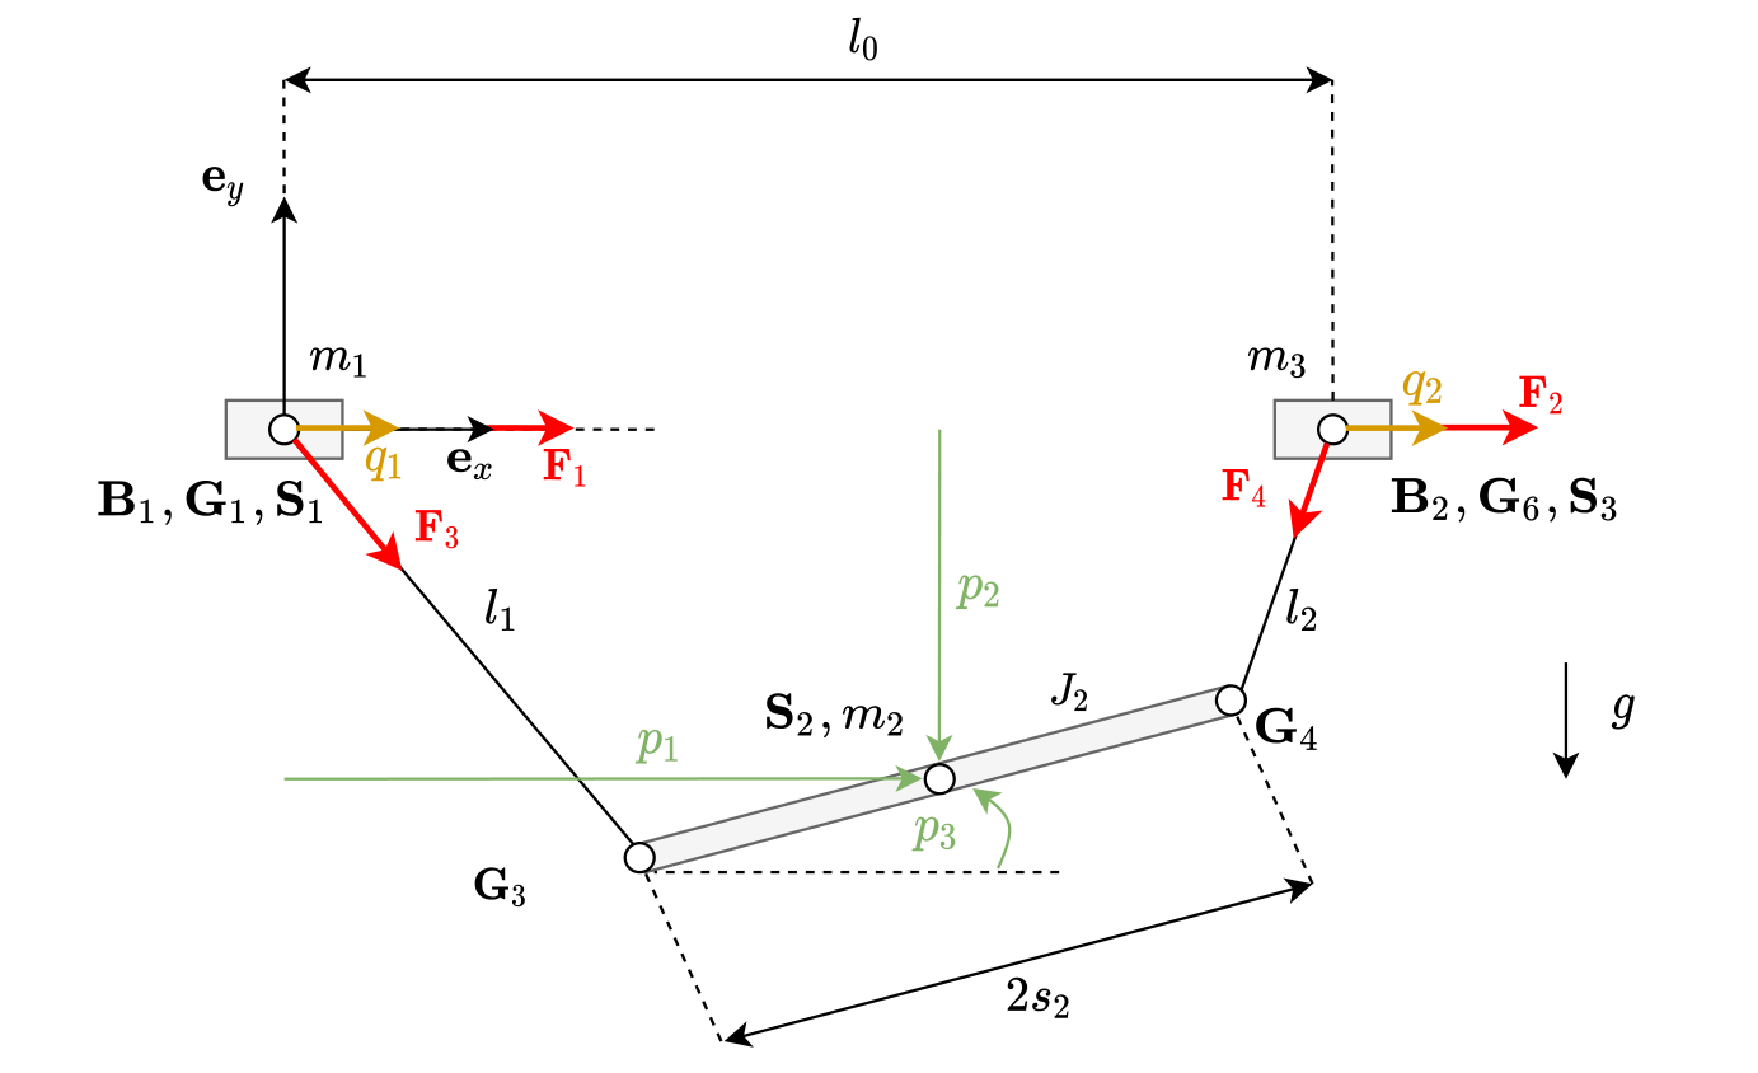
\includegraphics[width=90mm]{over_crane.pdf}
		\caption{Structure of the Overhead Crane. \\ 
		\footnotesize{Source: Wrede, Konstantin / Modellbildung und Reglerentwurf für ein Brückenkransystem }}
	\end{figure}

	
	%%%%%%%%%%%%%%%%%%%%%% MDOEL EQUATIONS %%%%%%%%%%%%%%%%%%%%%%%%%%%
	
	\section{Model Equations} % MUST
	
	State Vector and Input Vector:
	\begin{align*}
		\underline{x} &= (p_1 \ p_2 \ p_3 \ q_1 \ q_2 \ \dot{p}_1 \ \dot{p}_2 \ \dot{p}_3 \ \dot{q}_1 \ \dot{q}_2)^T\\
		&= (x_1 \ x_2 \ x_3 \ x_4 \ x_5 \ x_6 \ x_7 \ x_8 \ x_9 \ x_{10})^T \\
		\underline{u} &= (u_1 \ u_2 \ u_3 \ u_4)^T
	\end{align*}
	
	\noindent System Equations:			
	\begin{subequations}
	\begin{align}
		0 &= m_2 \ddot{x}_1 - \frac{u_4(-l_0 + s_2 \cos(x_3) + x_1 - x_5)}{l_2} - \frac{u_3(-s_2 \cos(x_3) + x_1 - x_4)}{l_1} \\
		0 &= gm_2 + m_2 \ddot{x}_2 - \frac{u_4(s_2 \sin(x_3) + x_2)}{l_2} - \frac{u_3(-s_2 \sin(x_3) + x_2)}{l_1} \\
		\begin{split}
		0 &= J_2 \ddot{x}_3 - \frac{s_2u_4(s_2 \sin(x_3) + x_2) \cos(x_3)}{l_2} + \frac{s_2u_4(-l_0 + s_2 \cos(x_3) + x_1 - x_5) \sin(x_3)}{l_2} \\\
		&+ \frac{s_2 u_3 (-s_2 \sin(x_3) + x_2) \cos(x_3)}{l_1} - \frac{s_2u_3(-s_2 \cos(x_3) + x_1 - x_4) \sin(x_3)}{l_1}
		\end{split} \\
		0 &= m_1 \ddot{x}_4 - u_1 + \frac{u_3(-s_2 \cos(x_3) + x_1 - x_4)}{l_1} \\
		0 &= m_3 \ddot{x}_5 - u_2 + \frac{u_4(-l_0 + s_2 \cos(x_3) + x_1 - x_5)}{l_2}
	\end{align}
	\end{subequations}

	%%%%%%%%%%%%%%%%%%%%%% PARAMETERS | OUTPUTS %%%%%%%%%%%%%%%%%%%%%%%%%%%
	\noindent
	Parameters: $s_1, m_1, m_2, m_3, J_2, l_0, l_1, l_2$ % variables with constant, predefined value
	\\
	Outputs: \underline{x} % MAY
	
	%%%%%%%%%%%%%%%%%%%%%% ASSUMPTIONS %%%%%%%%%%%%%%%%%%%%%%%%%%%
	
	\subsection{Assumptions} % MAY 
		\begin{enumerate} %possible list type for the Assumptions
			\item  The movement of all components is only considered in the vertical plane.
			\item The ropes are assumed to be massless.
			\item The load is considered to have a homogeneous mass distribution.
			\item Dissipative forces are not taken into account.
		\end{enumerate}
	
	%%%%%%%%%%%%%%%%%%%%%% EXEMPLARY PARAMETER VALUES %%%%%%%%%%%%%%%%%%%%%%%%%%%	
	
	\subsection{Exemplary parameter values}
	\begin{tabular}{cl}
\hline
  Symbol  & Value                                                                                                                                                                                \\
\hline
   $A$    & $\left[\begin{matrix}0.8189 & 0.0863 & 0.09 & 0.0813\\0.2524 & 1.0033 & 0.0313 & 0.2004\\-0.0545 & 0.0102 & 0.7901 & -0.258\\-0.1918 & -0.1034 & 0.1602 & 0.8604\end{matrix}\right]$ \\
   $B$    & $\left[\begin{matrix}0.0045 & 0.0044\\0.1001 & 0.01\\0.0003 & -0.0136\\-0.0051 & 0.0936\end{matrix}\right]$                                                                          \\
 $B_{1}$  & $\left[\begin{matrix}0.0045 & 0.0044\\0.1001 & 0.01\\0.0003 & -0.0136\\-0.0051 & 0.0936\end{matrix}\right]$                                                                          \\
 $C_{1}$  & $\left[\begin{matrix}1.0 & 0 & -1.0 & 0\\0 & 0 & 0 & 0\\0 & 0 & 0 & 0\end{matrix}\right]$                                                                                            \\
   $C$    & $\left[\begin{matrix}1.0 & 0 & 0 & 0\\0 & 0 & 1.0 & 0\end{matrix}\right]$                                                                                                            \\
 $D_{11}$ & $\left[\begin{matrix}0 & 0 & 0\\0 & 0 & 0\\0 & 0 & 0\end{matrix}\right]$                                                                                                             \\
 $D_{12}$ & $\left[\begin{matrix}0 & 0\\1.0 & 0\\0 & 1.0\end{matrix}\right]$                                                                                                                     \\
 $D_{21}$ & $\left[\begin{matrix}0 & 1.0 & 0\\0 & 0 & 1.0\end{matrix}\right]$                                                                                                                    \\
\hline
\end{tabular}

	%%%%%%%%%%%%%%%%%%%%%% DERIVATION & EXPLANATION %%%%%%%%%%%%%%%%%%%%%%%%%%%	
	
	\section{Derivation and Explanation} % SHOULD
	
	The Lagrangian mechanics was used for the solution.
	
	%%%%%%%%%%%%%%%%%%%%%% REFERENCES %%%%%%%%%%%%%%%%%%%%%%%%%%%
	
	\begin{thebibliography}{10}		
		\bibitem{Wrede}Wrede, Konstantin: 
		\textit{Modellbildung und Reglerentwurf für ein Brückenkransystem}, student research project at the Institut of Control Theory TU Dresden, published 2022. \\
		(not publicly accessible)
	\end{thebibliography}

\end{document}

